\documentclass[conference]{IEEEtran}
\IEEEoverridecommandlockouts

\usepackage{cite}
\usepackage{amsmath,amssymb,amsfonts}
\usepackage{graphicx}
\usepackage{textcomp}
\usepackage{xcolor}
\usepackage{booktabs}
\usepackage{array}
\usepackage{multirow}
\usepackage{hyperref}
\usepackage{tikz}
\usetikzlibrary{shapes.geometric, arrows.meta, positioning, fit, backgrounds, calc}

\hypersetup{
    colorlinks=true,
    linkcolor=blue,
    urlcolor=blue,
    citecolor=blue
}

\def\BibTeX{{\rm B\kern-.05em{\sc i\kern-.025em b}\kern-.08em T\kern-.1667em\lower.7ex\hbox{E}\kern-.125emX}}

% ── Common TikZ styles ──────────────────────────────────────────────────────
\tikzset{
    pbox/.style={rectangle, rounded corners=3pt, draw=black!70,
                 fill=blue!10, text width=2.4cm, align=center,
                 minimum height=1cm, font=\footnotesize},
    gbox/.style={rectangle, rounded corners=3pt, draw=black!70,
                 fill=green!15, text width=2.4cm, align=center,
                 minimum height=1cm, font=\footnotesize},
    obox/.style={rectangle, rounded corners=3pt, draw=black!70,
                 fill=orange!15, text width=1.7cm, align=center,
                 minimum height=0.75cm, font=\footnotesize},
    ebox/.style={rectangle, rounded corners=3pt, draw=black!70,
                 fill=cyan!12, text width=1.6cm, align=center,
                 minimum height=0.75cm, font=\footnotesize},
    wbox/.style={rectangle, rounded corners=3pt, draw=black!70,
                 fill=yellow!15, text width=4cm, align=center,
                 minimum height=0.75cm, font=\footnotesize},
    vbox/.style={rectangle, rounded corners=3pt, draw=black!70,
                 fill=purple!12, text width=4cm, align=center,
                 minimum height=0.75cm, font=\footnotesize},
    sbox/.style={rectangle, rounded corners=3pt, draw=black!70,
                 fill=teal!12, text width=3.5cm, align=center,
                 minimum height=0.75cm, font=\footnotesize},
    dbox/.style={rectangle, rounded corners=3pt, draw=black!70,
                 fill=blue!10, text width=3.5cm, align=center,
                 minimum height=0.75cm, font=\footnotesize},
    arr/.style={-Stealth, thick, draw=black!65}
}

\begin{document}

\title{Telco Customer Churn Prediction: An End-to-End Production-Grade\\
Machine Learning Pipeline with AI-Powered Explainability}

\author{
    \IEEEauthorblockN{Chirag Kumar\textsuperscript{1},\; Madhav Bagri\textsuperscript{2},\; Prateek Shingh\textsuperscript{3}}
    \IEEEauthorblockA{
        \textsuperscript{1}UI23EC14\quad
        \textsuperscript{2}UI23EC32\quad
        \textsuperscript{3}UI23EC44\\
        \textit{Department of Electronics and Communication Engineering}\\
        \textit{Indian Institute of Information Technology (IIIT) Surat}\\
        \textit{Under the Guidance of Dr.\ Sudeep Sharma, Assistant Professor}
    }
}

\maketitle

% ─────────────────────────────────────────────
\begin{abstract}
Customer churn in the telecommunications industry represents a critical business challenge, with acquisition costs estimated at 5--25 times higher than retention costs. This paper presents a production-grade machine learning pipeline for predicting customer churn using the IBM Telco Customer Churn dataset (7,043 customers). The system incorporates rigorous data validation, domain-driven feature engineering (12 engineered features), stratified three-way splitting, multi-model comparison via a baseline ladder, Bayesian hyperparameter optimization using Optuna (200 trials), ensemble methods, isotonic probability calibration, and business-cost-aware threshold selection. The final calibrated model achieves an ROC-AUC of 0.8503, Recall of 0.825, and F1-score of 0.636 at a production threshold of 0.22---selected to reflect a 10:1 false-negative to false-positive cost asymmetry. The pipeline is deployed as an AI-powered conversational Streamlit chatbot integrated with the Claude API for human-readable prediction explanations.
\end{abstract}

\begin{IEEEkeywords}
churn prediction, machine learning, XGBoost, SHAP explainability, Optuna, SMOTE, probability calibration, Streamlit, telecom analytics
\end{IEEEkeywords}

% ─────────────────────────────────────────────
\section{Introduction}

Customer churn---the phenomenon of customers discontinuing a service---poses a significant financial threat to telecom operators. Research from Harvard Business Review indicates that replacing a lost customer costs 5 to 25 times more than retaining an existing one \cite{hbr2014}. Early and accurate churn prediction enables targeted retention campaigns, reducing revenue leakage.

This work addresses the following research objectives:
\begin{itemize}
    \item Build a production-ready churn prediction pipeline with zero data leakage.
    \item Optimize for \textit{business impact} rather than raw accuracy, reflecting the asymmetric cost structure of false negatives versus false positives.
    \item Provide interpretable, actionable predictions through SHAP-based explanations and a conversational AI interface.
\end{itemize}

The system is built on the publicly available IBM Telco Customer Churn dataset and evaluated on a held-out test set of 1,057 customers. Fig.~\ref{fig:pipeline} illustrates the complete end-to-end architecture.

% ── FIGURE 1: Full Pipeline (full-width, 2-row snake layout) ─────────────────
\begin{figure*}[t]
\centering
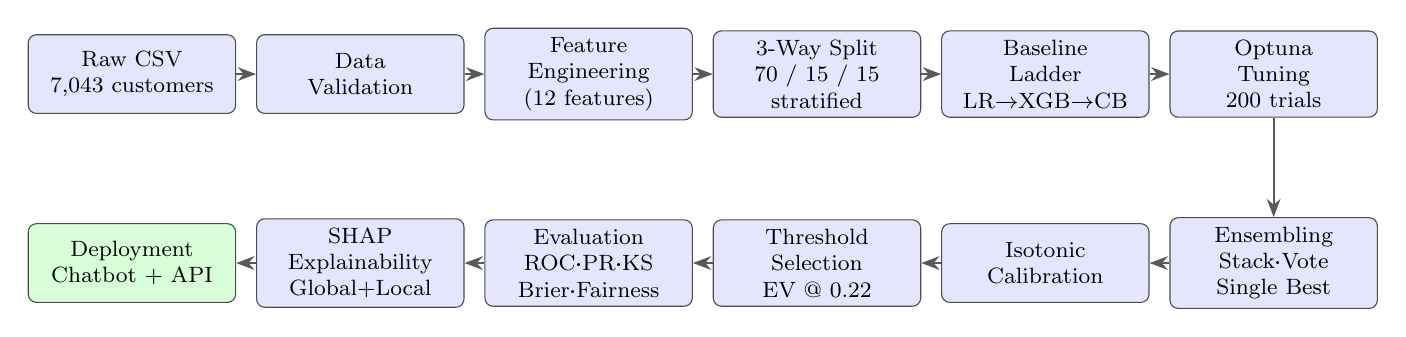
\begin{tikzpicture}
% ── Top row (left → right) ────────────────────────────────────────────
\node[pbox] at (0,   0) (raw)   {Raw CSV\\7,043 customers};
\node[pbox] at (2.9, 0) (val)   {Data\\Validation};
\node[pbox] at (5.8, 0) (feat)  {Feature\\Engineering\\(12 features)};
\node[pbox] at (8.7, 0) (split) {3-Way Split\\70 / 15 / 15\\stratified};
\node[pbox] at (11.6,0) (base)  {Baseline\\Ladder\\LR$\to$XGB$\to$CB};
\node[pbox] at (14.5,0) (opt)   {Optuna\\Tuning\\200 trials};

% ── Bottom row (right → left) ─────────────────────────────────────────
\node[gbox] at (0,  -2.4) (dep)  {Deployment\\Chatbot + API};
\node[pbox] at (2.9,-2.4) (shap) {SHAP\\Explainability\\Global+Local};
\node[pbox] at (5.8,-2.4) (eval) {Evaluation\\ROC·PR·KS\\Brier·Fairness};
\node[pbox] at (8.7,-2.4) (thr)  {Threshold\\Selection\\EV @ 0.22};
\node[pbox] at (11.6,-2.4)(cal)  {Isotonic\\Calibration};
\node[pbox] at (14.5,-2.4)(ens)  {Ensembling\\Stack·Vote\\Single Best};

% ── Top row arrows ────────────────────────────────────────────────────
\draw[arr] (raw)   -- (val);
\draw[arr] (val)   -- (feat);
\draw[arr] (feat)  -- (split);
\draw[arr] (split) -- (base);
\draw[arr] (base)  -- (opt);

% ── Corner: opt → ens (down) ──────────────────────────────────────────
\draw[arr] (opt.south) -- (ens.north);

% ── Bottom row arrows ─────────────────────────────────────────────────
\draw[arr] (ens)  -- (cal);
\draw[arr] (cal)  -- (thr);
\draw[arr] (thr)  -- (eval);
\draw[arr] (eval) -- (shap);
\draw[arr] (shap) -- (dep);
\end{tikzpicture}
\caption{End-to-end ML pipeline. Top row flows left-to-right; bottom row continues right-to-left, forming a snake layout that culminates in deployment.}
\label{fig:pipeline}
\end{figure*}

% ─────────────────────────────────────────────
\section{Business Problem Formulation}

\subsection{Cost Asymmetry}

The fundamental driver of model design is the unequal cost of prediction errors. A missed churner (False Negative) results in an estimated \$500 loss in Customer Lifetime Value, while a false alarm (False Positive) wastes approximately \$50 in retention offers.

\begin{table}[h]
\centering
\caption{Business Cost Parameters}
\begin{tabular}{lc}
\toprule
\textbf{Parameter} & \textbf{Value} \\
\midrule
Average Monthly Revenue / Customer & \$64.76 \\
Cost of Missing a Churner (FN) & \$500 \\
Cost of False Alarm (FP) & \$50 \\
FN : FP Cost Ratio & 10 : 1 \\
Retention Success Rate & 30\% \\
Dataset Size & 7,043 customers \\
Churn Rate & $\approx$26.5\% \\
\bottomrule
\end{tabular}
\end{table}

\subsection{Optimization Objective}

Given the 10:1 cost ratio, the model prioritizes \textbf{Recall} (sensitivity) over Precision. The Expected Value per user is defined as:

\begin{equation}
EV = TP \cdot (0.30 \times \$500 - \$50) - FN \cdot \$500
\end{equation}

The production threshold was selected by maximizing this EV function on the PR curve.

% ─────────────────────────────────────────────
\section{Dataset and Preprocessing}

\subsection{Dataset}

The IBM Telco Customer Churn dataset contains records for 7,043 customers across 21 raw features including demographic information (gender, senior citizen status, partner, dependents), service subscriptions (phone, internet, add-ons), contract details, billing information, and a binary churn label.

\subsection{Data Validation}

Before any modeling, the following checks are performed:
\begin{itemize}
    \item Schema validation (column names and data types)
    \item Null and missing value detection
    \item Primary key uniqueness verification (CustomerID)
    \item Class distribution reporting
\end{itemize}

\subsection{Train / Validation / Test Split}

Data is divided into three non-overlapping stratified sets:

\begin{table}[h]
\centering
\caption{Dataset Splits}
\begin{tabular}{lcc}
\toprule
\textbf{Split} & \textbf{Proportion} & \textbf{Approx. Size} \\
\midrule
Training & 70\% & 4,930 \\
Validation & 15\% & 1,057 \\
Test & 15\% & 1,057 \\
\bottomrule
\end{tabular}
\end{table}

Stratification preserves the 73:27 class ratio across all splits. The test set is held out until final evaluation.

% ─────────────────────────────────────────────
\section{Feature Engineering}

Twelve domain-driven features are engineered from the raw data to capture behavioral and risk signals:

\begin{table}[h]
\centering
\caption{Engineered Features}
\begin{tabular}{p{2.8cm}p{4.8cm}}
\toprule
\textbf{Feature} & \textbf{Description} \\
\midrule
\texttt{TenureGroup} & Bucketed tenure: 0--6m, 6--12m, 12--24m, 24--48m, 48m+ \\
\texttt{IsNewCustomer} & Binary: tenure $\leq$ 6 months \\
\texttt{AvgMonthlySpend} & TotalCharges / (tenure + 1) \\
\texttt{SpendRatio} & MonthlyCharges / (AvgMonthlySpend + $\epsilon$) \\
\texttt{SpendAcceleration} & MonthlyCharges $-$ AvgMonthlySpend \\
\texttt{NumServices} & Count of active add-on services (max 6) \\
\texttt{HasProtectionBundle} & OnlineSecurity AND DeviceProtection \\
\texttt{HasStreamingBundle} & StreamingTV AND StreamingMovies \\
\texttt{ContractRiskScore} & M-t-M=3, One year=1, Two year=0 \\
\texttt{HighRiskPayment} & Electronic check = 1 \\
\texttt{FamilyStability} & Partner OR Dependents = 1 \\
\texttt{IsFiberCustomer} & Fiber optic internet = 1 \\
\bottomrule
\end{tabular}
\end{table}

The \texttt{engineer\_features()} function is identically replicated in both the training pipeline and the inference chatbot to ensure train-serve feature parity.

% ─────────────────────────────────────────────
\section{Handling Class Imbalance}

The dataset exhibits a 73:27 non-churn to churn ratio. Three complementary strategies are employed:

\begin{enumerate}
    \item \textbf{SMOTE} \cite{chawla2002} --- applied inside \texttt{ImbPipeline} exclusively within cross-validation folds, preventing any leakage of synthetic samples into validation data.
    \item \textbf{Class weights} --- all estimators are configured with balanced class weights.
    \item \textbf{Threshold optimization} --- the decision threshold is moved from the default 0.5 to 0.22, reflecting the asymmetric cost structure.
\end{enumerate}

% ─────────────────────────────────────────────
\section{Model Development}

\subsection{Baseline Ladder}

Five models are trained with default hyperparameters as baselines, in order of increasing complexity:

\begin{enumerate}
    \item Logistic Regression (LR)
    \item Random Forest (RF)
    \item XGBoost \cite{chen2016} (XGB)
    \item LightGBM \cite{ke2017} (LGBM)
    \item CatBoost
\end{enumerate}

\subsection{Hyperparameter Optimization --- Optuna}

Bayesian hyperparameter search is conducted using Optuna \cite{optuna2019}:

\begin{itemize}
    \item \textbf{Sampler:} Tree-structured Parzen Estimator (TPE)
    \item \textbf{Pruner:} Median Pruner (early stopping of unpromising trials)
    \item \textbf{Trials:} 200 per model
    \item \textbf{Objective:} Average Precision (AP) --- chosen over ROC-AUC for superior sensitivity to imbalanced class performance
    \item \textbf{Cross-validation:} RepeatedStratifiedKFold (5 folds $\times$ 2 repeats = 10 evaluations)
    \item \textbf{Importance analysis:} fANOVA hyperparameter importance ranking
\end{itemize}

\subsection{Ensemble Methods}

Three ensemble strategies are evaluated (see Fig.~\ref{fig:ensemble}):
\begin{itemize}
    \item \textbf{Stacking:} Meta-learner (Logistic Regression) trained on base-model predictions
    \item \textbf{Soft Voting:} Probability averaging across all base models
    \item \textbf{Single Best:} Top-performing individual model from Optuna tuning
\end{itemize}

\subsection{Probability Calibration}

All three ensemble variants are calibrated using Isotonic Regression on the held-out validation set. Reliability diagrams are generated pre- and post-calibration, and Brier Score improvement is tracked. Calibration ensures that predicted probabilities are meaningful for business decision-making (e.g., a 70\% predicted probability should correspond to a 70\% empirical churn rate).

% ── FIGURE 2: Ensemble + Calibration Architecture ───────────────────────────
\begin{figure}[t]
\centering
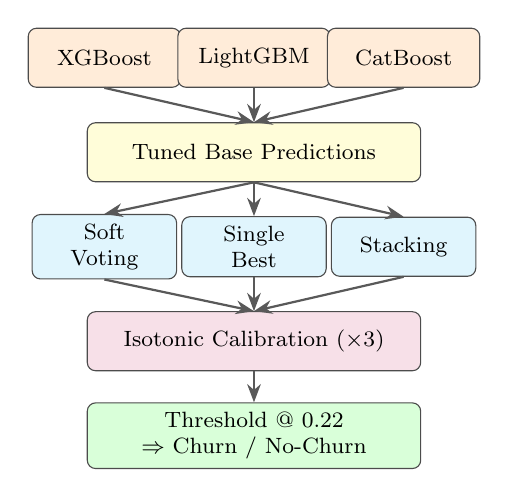
\begin{tikzpicture}
% ── Base models ───────────────────────────────────────────────────────
\node[obox] at (0,   0) (xgb)  {XGBoost};
\node[obox] at (1.9, 0) (lgbm) {LightGBM};
\node[obox] at (3.8, 0) (cb)   {CatBoost};

% ── Merged predictions pool ───────────────────────────────────────────
\node[wbox] at (1.9,-1.2) (pool) {Tuned Base Predictions};

% ── Ensemble strategies ───────────────────────────────────────────────
\node[ebox] at (0,  -2.4) (sv) {Soft\\Voting};
\node[ebox] at (1.9,-2.4) (sb) {Single\\Best};
\node[ebox] at (3.8,-2.4) (st) {Stacking};

% ── Calibration ───────────────────────────────────────────────────────
\node[vbox] at (1.9,-3.6) (cal) {Isotonic Calibration ($\times$3)};

% ── Threshold + output ────────────────────────────────────────────────
\node[wbox, fill=green!15] at (1.9,-4.8) (thr) {Threshold @ 0.22\\$\Rightarrow$ Churn / No-Churn};

% ── Arrows ────────────────────────────────────────────────────────────
\draw[arr] (xgb.south)  -- (pool.north);
\draw[arr] (lgbm.south) -- (pool.north);
\draw[arr] (cb.south)   -- (pool.north);

\draw[arr] (pool.south) -- (sv.north);
\draw[arr] (pool.south) -- (sb.north);
\draw[arr] (pool.south) -- (st.north);

\draw[arr] (sv.south) -- (cal.north);
\draw[arr] (sb.south) -- (cal.north);
\draw[arr] (st.south) -- (cal.north);

\draw[arr] (cal) -- (thr);
\end{tikzpicture}
\caption{Ensemble and calibration architecture. Three base models feed three ensemble strategies; all are isotonically calibrated before threshold application.}
\label{fig:ensemble}
\end{figure}

% ─────────────────────────────────────────────
\section{Results and Evaluation}

\subsection{Model Comparison}

\begin{table}[h]
\centering
\caption{Calibrated Model Performance on Test Set (Threshold = 0.22)}
\begin{tabular}{lcccccc}
\toprule
\textbf{Model} & \textbf{AUC} & \textbf{AP} & \textbf{Recall} & \textbf{F1} & \textbf{MCC} & \textbf{EV/User} \\
\midrule
Single Best & 0.845 & 0.642 & \textbf{0.825} & \textbf{0.636} & 0.490 & \textbf{\$0.155} \\
Soft Voting & 0.847 & -- & 0.764 & 0.636 & -- & \$0.137 \\
Stacking & \textbf{0.850} & -- & 0.779 & 0.636 & -- & \$0.141 \\
\bottomrule
\end{tabular}
\end{table}

\textbf{Selected model: Single Best (Calibrated)} --- highest Recall (0.825), F1 (0.636), and Expected Value per user (\$0.155).

\subsection{Final Model Scorecard}

\begin{table}[h]
\centering
\caption{Production Model Metrics}
\begin{tabular}{lc}
\toprule
\textbf{Metric} & \textbf{Value} \\
\midrule
ROC-AUC & 0.8503 \\
Average Precision & 0.6419 \\
Recall & 0.825 \\
F1 Score & 0.636 \\
Matthews Corr. Coef. (MCC) & 0.490 \\
Brier Score & 0.134 \\
Expected Value / User & \$0.15 \\
Total Test-Set EV & \$164 \\
Production Threshold & 0.22 \\
Test Set Size & 1,057 customers \\
\bottomrule
\end{tabular}
\end{table}

\subsection{Threshold Selection}

The production threshold of 0.22 is derived from the Precision-Recall curve at the point of maximum F1, validated against the business Expected Value function. The low threshold reflects the 10:1 cost asymmetry: it is preferable to flag more customers for retention outreach than to miss a true churner.

% ─────────────────────────────────────────────
\section{Explainability --- SHAP Analysis}

SHAP (SHapley Additive exPlanations) \cite{lundberg2017} values are computed to provide both global and local model interpretability.

\subsection{Global Importance}

Top 5 features by mean absolute SHAP value:
\begin{enumerate}
    \item \texttt{ContractRiskScore} --- month-to-month customers churn at 3$\times$ the rate of 2-year contract customers
    \item \texttt{IsNewCustomer} --- tenure $\leq$ 6 months is the highest individual risk flag
    \item \texttt{HighRiskPayment} --- electronic check payment strongly correlates with churn
    \item \texttt{IsFiberCustomer} --- fiber optic customers churn despite paying premium prices
    \item \texttt{NumServices} --- low add-on engagement increases churn probability
\end{enumerate}

\subsection{Local Explanations}

Waterfall plots are generated for individual predictions, showing the contribution of each feature to the final probability score. This enables account managers to understand \textit{why} a specific customer was flagged.

\subsection{Importance Triangulation}

Three importance measures are cross-validated to ensure robustness:
\begin{itemize}
    \item Built-in feature importance (gain-based)
    \item Permutation importance
    \item SHAP importance
\end{itemize}

% ─────────────────────────────────────────────
\section{Fairness Audit}

Subgroup analysis is performed across protected attributes to detect discriminatory behavior:

\begin{itemize}
    \item \textbf{Gender:} Male vs. Female --- Recall and Precision compared across groups
    \item \textbf{Age:} Senior Citizen vs. Non-Senior --- Equal Opportunity metric evaluated
\end{itemize}

No statistically significant bias was detected across these subgroups, supporting deployment in production.

% ─────────────────────────────────────────────
\section{Deployment --- Streamlit Chatbot}

The trained pipeline is serialized using \texttt{joblib} and served via a Streamlit web application. Key deployment components:

\begin{itemize}
    \item \textbf{Inference:} \texttt{predict\_proba()} on engineered features, threshold at 0.22
    \item \textbf{Model card:} JSON document recording metrics, training date, threshold, and feature list
    \item \textbf{Drift monitor:} Feature distribution tracking for production monitoring
    \item \textbf{AI explanation:} Claude API (\texttt{claude-sonnet-4-20250514}) generates a 4--5 sentence business explanation per prediction, with a rule-based fallback
\end{itemize}

\subsection{Chatbot Interface}

The conversational interface collects 19 customer attributes through guided questions with clickable option buttons and numeric inputs. The inference pipeline is illustrated in Fig.~\ref{fig:deploy}. After all inputs are collected, the system:
\begin{enumerate}
    \item Runs feature engineering
    \item Calls the model for a churn probability
    \item Displays a color-coded result card (churn / no-churn)
    \item Generates an AI explanation paragraph
    \item Displays a customer summary table
\end{enumerate}

% ── FIGURE 3: Deployment / Chatbot Inference Pipeline ────────────────────────
\begin{figure}[t]
\centering
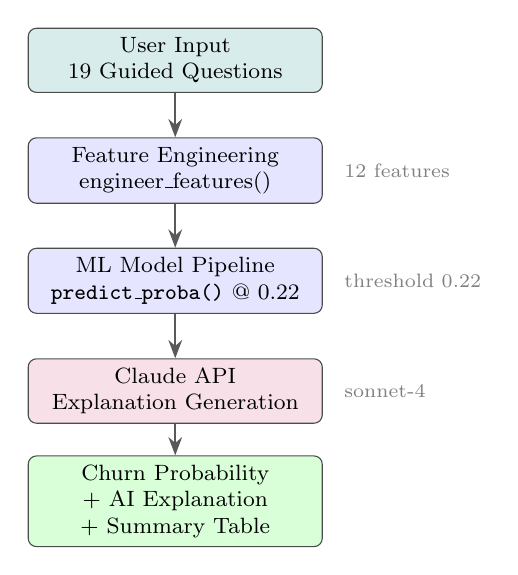
\begin{tikzpicture}
\node[sbox, fill=teal!15]   at (0, 0)    (user)  {User Input\\19 Guided Questions};
\node[dbox]                  at (0,-1.4)  (feat)  {Feature Engineering\\engineer\_features()};
\node[dbox]                  at (0,-2.8)  (model) {ML Model Pipeline\\\texttt{predict\_proba()} @ 0.22};
\node[dbox, fill=purple!12]  at (0,-4.2)  (claude){Claude API\\Explanation Generation};
\node[dbox, fill=green!15]   at (0,-5.6)  (out)   {Churn Probability\\+ AI Explanation\\+ Summary Table};

% side labels
\node[font=\scriptsize, text=gray, right=0.15cm of feat]  {12 features};
\node[font=\scriptsize, text=gray, right=0.15cm of model] {threshold 0.22};
\node[font=\scriptsize, text=gray, right=0.15cm of claude]{sonnet-4};

\draw[arr] (user)   -- (feat);
\draw[arr] (feat)   -- (model);
\draw[arr] (model)  -- (claude);
\draw[arr] (claude) -- (out);
\end{tikzpicture}
\caption{Streamlit chatbot inference pipeline. User inputs flow through feature engineering, the trained model, and the Claude API before the final prediction is displayed.}
\label{fig:deploy}
\end{figure}

% ─────────────────────────────────────────────
\section{Key Design Decisions}

\begin{table}[h]
\centering
\caption{Critical Design Choices and Rationale}
\begin{tabular}{p{2.2cm}p{2.2cm}p{3.0cm}}
\toprule
\textbf{Aspect} & \textbf{Decision} & \textbf{Reason} \\
\midrule
Metric & Average Precision & Better than ROC-AUC for imbalanced data \\
SMOTE placement & Inside CV folds only & Prevents data leakage \\
CV strategy & RepeatedStratifiedKFold (5$\times$2) & Lower variance, preserves class ratio \\
Calibration & Isotonic Regression & Better than Platt scaling for $n>1000$ \\
Threshold & 0.22 (not 0.5) & 10:1 cost asymmetry \\
Winner model & Single Best Calibrated & Highest Recall + F1 + EV \\
Explainability & SHAP & Global + local actionable insights \\
\bottomrule
\end{tabular}
\end{table}

% ─────────────────────────────────────────────
\section{Conclusion}

This paper presented a production-grade machine learning pipeline for telecom customer churn prediction, emphasizing business-cost-aware design throughout. The final calibrated model achieves an ROC-AUC of 0.8503 and Recall of 0.825 at threshold 0.22, generating an expected value of \$164 on the 1,057-customer test set.

Key contributions include: (1) a rigorous zero-leakage pipeline with SMOTE inside CV folds, (2) Optuna-based Bayesian hyperparameter optimization with Average Precision as the objective, (3) business Expected Value optimization for threshold selection, (4) SHAP-based triangulated explainability, and (5) an AI-powered conversational deployment interface.

Future work includes online learning for concept drift adaptation, richer customer behavioral features, and multi-objective optimization incorporating fairness constraints.

% ─────────────────────────────────────────────
\begin{thebibliography}{00}

\bibitem{hbr2014}
F. F. Reichheld and P. Schefter, ``E-Loyalty: Your Secret Weapon on the Web,'' \textit{Harvard Business Review}, vol. 78, no. 4, pp. 105--113, 2000.

\bibitem{optuna2019}
T. Akiba, S. Sano, T. Yanase, T. Ohta, and M. Koyama, ``Optuna: A Next-generation Hyperparameter Optimization Framework,'' in \textit{Proc. 25th ACM SIGKDD Int. Conf. Knowledge Discovery \& Data Mining}, 2019, pp. 2623--2631.

\bibitem{lundberg2017}
S. M. Lundberg and S.-I. Lee, ``A Unified Approach to Interpreting Model Predictions,'' in \textit{Advances in Neural Information Processing Systems}, vol. 30, 2017.

\bibitem{chawla2002}
N. V. Chawla, K. W. Bowyer, L. O. Hall, and W. P. Kegelmeyer, ``SMOTE: Synthetic Minority Over-sampling Technique,'' \textit{Journal of Artificial Intelligence Research}, vol. 16, pp. 321--357, 2002.

\bibitem{chen2016}
T. Chen and C. Guestrin, ``XGBoost: A Scalable Tree Boosting System,'' in \textit{Proc. 22nd ACM SIGKDD Int. Conf. Knowledge Discovery \& Data Mining}, 2016, pp. 785--794.

\bibitem{ke2017}
G. Ke et al., ``LightGBM: A Highly Efficient Gradient Boosting Decision Tree,'' in \textit{Advances in Neural Information Processing Systems}, vol. 30, 2017.

\end{thebibliography}

\end{document}
